\begin{egBox}{Not all Subsets of a Compact Space are Compact}[eg:26.1]
    We shall consider the open covers of the circle \( S \) and of the circle
    minus its north pole.

    \begin{figure}[H]
        \centering
        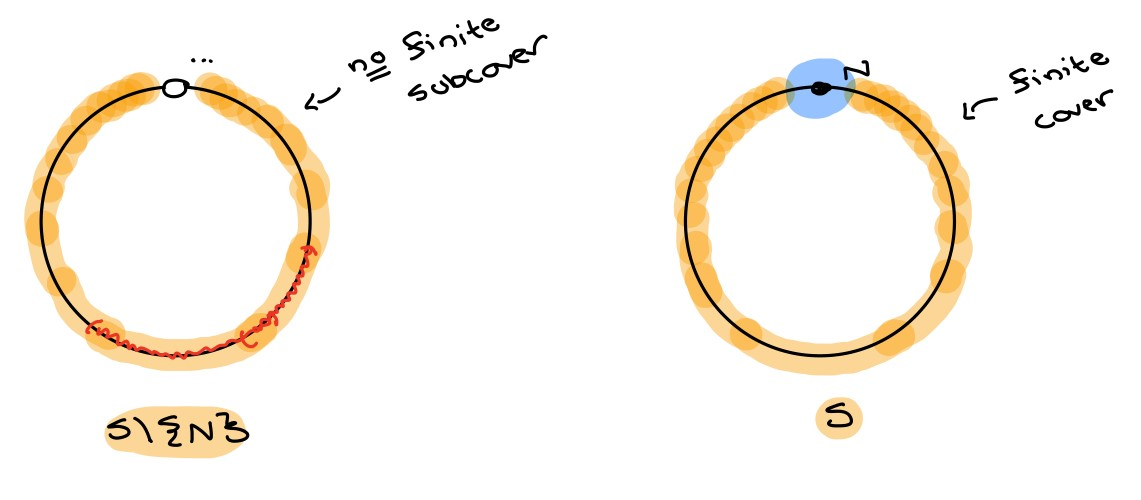
\includegraphics[ width = 0.7\linewidth ]{figures/Section 26/26_eg1.jpg}
        \caption{The two subspaces in question}
        \label{fig:26-3}
    \end{figure}

    For the circle minus its north pole, we can construct a cover by 
    adding smaller and smaller open sets of the circle such that it eventually 
    approaches the north pole, but never reaches it.

    \baseSkip

    For the circle with the north pole, we see that we can use the same cover
    as above, but with another open set that contains the north pole.
    In fact, we see that the open set that contains the north pole
    contains infinitely many other open sets that are in the cover,
    Thus, we see that such sets are redundant, meaning that we can remove them
    from our cover.
    What results is that we get a finite cover on the circle.

    \baseSkip

    However, for the circle without the north pole, we see that there cannot 
    exist a finite subcover -- the infinite open sets that lead up to the north
    pole were vital towards our cover for this subspace.

    \baseSkip

    This example tells us that not all subsets of a compact set are compact;
    the condition that sets be closed was key being able to avoid a situation
    where there were infinite open sets that led up to a limit point (in our 
    case, the north pole).
\end{egBox}

\begin{egBox}{Compact Sets in the Cofinite Topology}[eg:26.2]
    Let \( X \) be a set equipped with the cofinite topology.
    Prove that every subset of \( X \) is compact in \( X \).

    \baseSkip

    Let \( A \) be any subset of \( X \).
    Let \( \mathcal{U} = \{ U_{ i } \}_{ i \in I } \) be any open cover of 
    \( A \).
    Our goal is to show that there exists a finite subcollection of 
    \( \mathcal{U} \) that covers \( A \).

    \baseSkip

    Let us focus on \( U_{ i } \) for some fixed index \( i \in I \).
    Since \( X \) is equipped with the cofinite topology, we have that 
    \( U_{ i } \) being open implies that \( X \setminus U_{ i } \) is finite.
    I.e., we see that there are only finitely many points in \( X \) that 
    are \textit{not} contained in \( U_{ i } \).
    In particular, this means that there are finitely many points in \( A \)
    that are not contained in \( U_{ i } \); in the case that all points of 
    \( A \) are in \( U_{ i } \), then we have that \( A \) is compact since
    \( U_{ i } \) itself is a finite subcover of \( A \).
    Let's say that \( x_{ 1 } , \ldots , x_{ n } \) are the points in \( A \)
    that are \textit{not} contained in \( U_{ i } \).
    Because \( \mathcal{U} \) is an open cover of \( A \), each of the points 
    \( x_{ 1 } , \ldots , x_{ n } \) are contained in some open set 
    \( \{ U_{ i_{ 1 } } , \ldots , U_{ i_{ n } } \} \) in the cover.

    \baseSkip

    Thus, we see that 
    \begin{equation*}
        \{ U_{ i }, U_{ i_{ 1 } } , \ldots , U_{ i_{ n } } \}
    \end{equation*}
    is a finite subcollection of \( \mathcal{U} \) that covers \( A \).
    Hence, \( A \) is compact in \( X \).
\end{egBox}

\begin{egBox}{Tubular Neighborhoods}[eg:26.3]
    We give an open neighborhood of \( \mathbb{R} \times \{ 0 \} \)

    \begin{figure}[H]
        \centering
        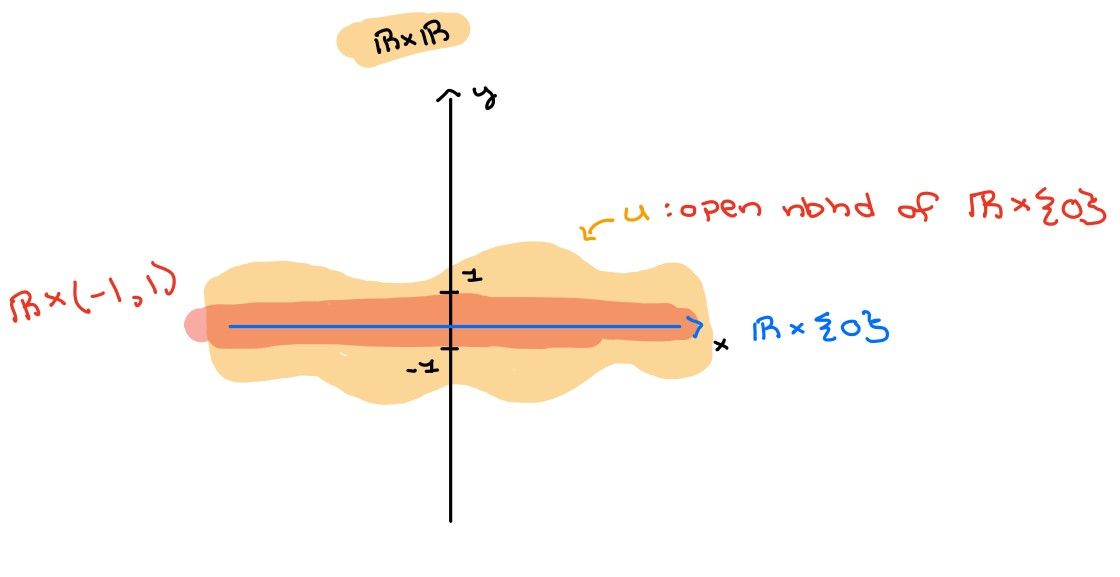
\includegraphics[ width = 0.6\linewidth ]{figures/Section 26/26_eg3.jpg}
        \caption{An example of a tubular neighborhood}
        \label{fig:26-4}
    \end{figure}

    However, not all neighborhoods of \( \mathbb{R} \times \{ 0 \} \) 
    contain a tubular neighborhood:

    \begin{figure}[H]
        \centering
        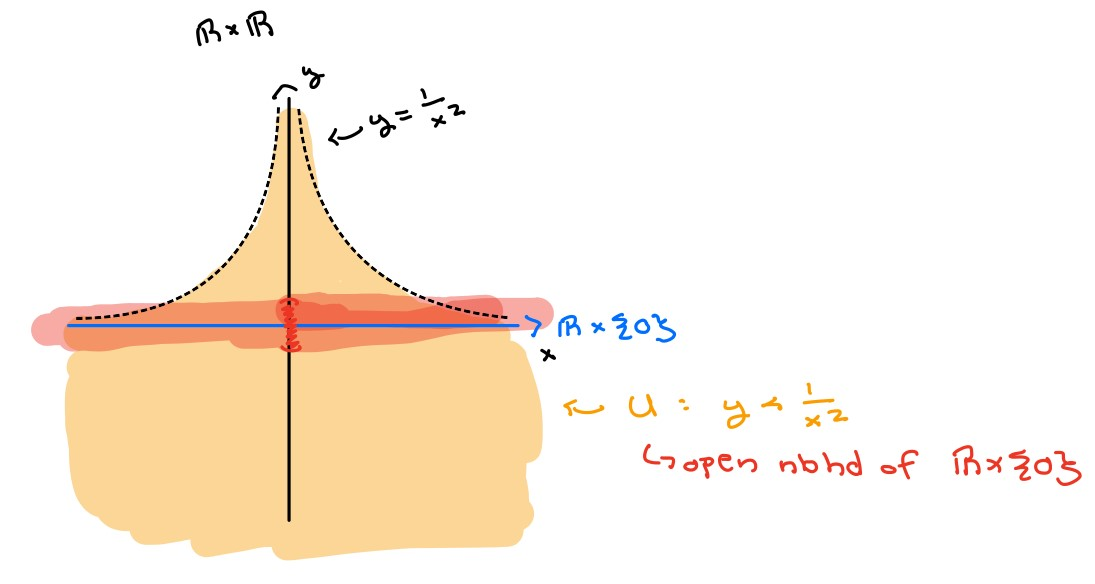
\includegraphics[ width = 0.6\linewidth ]{figures/Section 26/26_eg3-2.jpg}
        \caption{An example where no tubular neighborhoods exist}
        \label{fig:26-5}
    \end{figure}
\end{egBox}